\documentclass{iwsm}

\usepackage[numbers, sectionbib]{natbib}
\usepackage[utf8]{inputenc} % allow utf-8 input
\usepackage{hyperref}       % hyperlinks
\usepackage{url}            % simple URL typesetting
\usepackage{booktabs}       % professional-quality tables
\usepackage{amsfonts}       % blackboard math symbols
\usepackage{nicefrac}       % compact symbols for 1/2, etc.
\usepackage{microtype}      % microtypography
\usepackage{xcolor}         % colors
\usepackage{tikz}
\usetikzlibrary{arrows}
\usepackage{amsmath}
\usepackage{mathtools}
\usepackage{bbm}
\usepackage{amssymb}
\usepackage{algorithm}
\usepackage{algpseudocode}
\usepackage{caption}
\usepackage{subcaption}
\usepackage{graphicx}
\usepackage{float}
\usepackage{placeins}
\usepackage{enumitem}

%images
\graphicspath{{./img/}}


%bibliography
\bibliographystyle{splncs04}


\title{The Feature-First Block Model}

\author{Lawrence Tray \inst{1} \and Ioannis Kontoyiannis \inst{2}}

\institute{Department of Engineering, University of Cambridge, \email{lpt30@cantab.ac.uk} \and 
Statistical Laboratory, University of Cambridge, \email{yiannis@maths.cam.ac.uk}}

%custom commands
\DeclareMathOperator*{\argmax}{arg\,max} % Jan Hlavacek
\DeclareMathOperator*{\argmin}{arg\,min} % Jan Hlavacek

\def\imagebox#1#2{\vtop to #1{\null\hbox{#2}\vfill}}


\begin{document}
	
	\maketitle
	
	\begin{abstract}
	Labelled networks are an extremely common and important form of data. A typical inference goal is to determine how the vertex labels (called features) affect graphical structure. The standard approach to this problem is to partition the network into blocks grouped by distinct values of the feature of interest. We then use a block-based random graph model - typically a variant of the stochastic block model (SBM) - to test for evidence these extracted feature-based communities interact differently with one another.
	
	Nevertheless, these feature-based communities are often not a natural partition of the graph and thus the model is not a good fit. With this in mind, we present a novel generative model, which we call the feature-first block model (FFBM), for better describing vertex-labelled undirected graphs. We present a method to efficiently sample the FFBM parameters. This allows us to automatically determine which features best explain the block-based graphical structure. Importantly, this analysis can be performed using the whole feature-set rather than considering each feature independently. 
	
	We apply the developed method to a variety of network data to extract the most important features along which the vertices cluster. Those that do not impact the high-level structure can be discarded to reduce the problem dimension. In the case the vertex features available do not readily explain the community structure in the resulting network, the approach detects this and is protected against over-confidence. Future work may benefit from extending the FFBM to multiple hierarchical levels. This allows the structure to be explained at each level of coarseness. 
\end{abstract}

	\section{Introduction}

Many real-world networks exhibit strong community structure, with most nodes belonging to densely connected clusters. 
In this work, we examine vertex-labelled networks, 
referring to the labels as {\em features}. A typical goal is to determine whether a given feature impacts graphical structure. Answering this requires a random graph model;
the standard is the stochastic block model (SBM) -- see Peixoto (2017).

Analysing a labelled network with a simple SBM variant, requires partitioning the graph into blocks grouped by distinct values of the feature of interest. The associated model can then be used to test for evidence of heterogeneous connectivity between the feature-grouped blocks. Nevertheless, this approach can only consider disjoint feature sets and the feature-grouped blocks are often an unnatural partition of the graph.

We would instead prefer to partition the graph into its most natural blocks and then find which of the available features -- if any -- best predict the resulting partition. Thus motivated, we present a novel framework for modelling labelled networks.
This is not the first extension of the SBM to labelled networks, e.g. Stanley et al (2019). However, most of the current approaches are focused on leveraging feature information to partition the graph more reliably in the presence of noise.
We seek instead to develop a model well suited for inferring how vertex features impact graphical structure and to report our confidence in those conclusions.

	\section{Preliminaries}

This section defines some preliminary concepts required for the subsequent analysis. We first need a model for community-like structure in a graphical network. For this we adopt the stochastic block model (SBM) - widely used across academia. The premise is that each node in the graph belongs to a unique community called a block. The probability that two nodes are connected depends only on the block memberships of each. Graphs drawn from the SBM ensemble exhibit community structure. Specifically, we will use the microcanonical variant of the SBM, proposed by \citet{Peixoto-Bayesian-Microcanonical}. A paraphrased definition is given below for the non-degree-corrected SBM (NDC-SBM).

\begin{definition}[Microcanonical NDC-SBM]
	\label{defn:microcan-ndc-sbm}
	Let $N \in \Integers^{+}$ denote the number of vertices in an undirected graph. The block memberships are encoded by a vector $b$ of length $N$ where each entry $b_i \in \{1, 2 \dots B\}$. $B \in \Integers^{+}$ is the number of non-empty blocks. Let $e$ be a $B \times B$ matrix of edge counts between blocks ($e_{rs}$ is number of edges from block $r$ onto block $s$ - or twice that number if $r=s$). For undirected graphs $e$ is symmetric. For a non-degree-corrected stochastic block model (NDC-SBM), we say that the graph $A$ is generated as follows:
	%
	\begin{equation}
		A \sim \textrm{NDC-SBM}_{\textrm{MC}} (b, e)
	\end{equation}
	%
	Where edges are placed uniformly at random but respecting the constraint imposed by $e$ and $b$. The additional parameters $N$ and $B$ are omitted as they are inferred from the shapes of $b$ and $e$. If we interpret $A$ as an adjacency matrix, then this constraint can be written formally as: $e_{rs} = \sum_{i,j} A_{ij} \one \{b_i = r\} \one \{b_j = s\}$.
\end{definition}

Nevertheless, this formulation does not accept high degree variability within blocks as is typical of real-world data. Indeed, the NDC-SBM favours a partition into high-degree and low-degree nodes rather than clusters of inter-connected nodes. We therefore introduce the degree-corrected SBM (DC-SBM) \cite{Peixoto-Bayesian-Microcanonical} to circumvent these issues. 

\begin{definition}[Microcanonical DC-SBM]
	\label{defn:microcan-dc-sbm}
	This is much like the NDC-SBM but has an additional parameter $k$ which is an $N$-length vector encoding the degree sequence ($k_i$ is the degree of vertex $i$). Therefore, we write:
	%
	\begin{equation}
		A \sim \textrm{DC-SBM}_{\textrm{MC}} (b, e, k)
	\end{equation}
	%
	Once again, edges are placed uniformly at random but respecting the constraints imposed by the parameters. The DC-SBM has the additional constraint that $k_i = \sum_{j} A_{ij}$. In what follows, we will always assume the degree-corrected model unless otherwise specified.
	
\end{definition}
	\section{Feature-first block model}

In this section we propose a novel generative model for labelled networks. We call this the feature-first block model (FFBM) and outline its structure in \ref{fig:ffbm} As before, we let $N$ denote the number of nodes and $B$ the number of blocks in our graph. We define the vector $x_i \in \Xcal^D$ as the feature vector for the $i$'th vertex. $D$ is the number of features. For the datasets we analyse, we deal with binary feature flags so $\Xcal = \{0, 1\}$. The feature vectors $\{x_i\}_{i=1}^{N}$ may be compactly subsumed into the feature matrix $X \in \Xcal^{N \times D}$.

For the FFBM, we start with the feature matrix X and probabilistically generate a vector of block memberships $b \in [B]^N$. The parameters of this step are encapsulated by $\theta$. Each feature vector $x_i$ is treated independently and used to generate the corresponding block membership $b_i \in [B]$. We choose a single softmax layer to model $p(b_i | x_i, \theta)$. More complex models are possible but then deriving meaning from the inferred parameter distributions is more difficult. Summarising, we write $p(b | X, \theta)$ as follows:
%
\begin{equation}
	p(b| X, \theta) = \prod_{i=1}^{N} p(b_i | x_i, \theta) = \prod_{i=1}^{N} \phi_{b_i} (x_i; \theta)
	= \prod_{i=1}^{N} \frac{\exp\left(w_{b_i}^T x_i\right)}{\sum_{k=1}^{B} \exp \left( w_k^T x_i\right)}
\end{equation}
%
We deliberately exclude a bias term to ensure that the relationships we model are based on features and not information about the size of each detected block; a more complete discussion on this topic is given in \ref{appdx:dimension}. The parameter vector $\theta$ for this stage contains all the weight vectors $\theta = \{w_k\}_{k=1}^{B}$. Each $w_k$ has dimension $D$. We could instead write the parameters $\theta$ as a $B \times D$ matrix of weights $W$; this form has computational benefits as then $z_i \coloneqq W x_i$, which is the input to the softmax activation function.

\begin{figure}[!h]
	\centering
	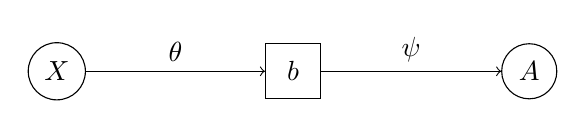
\begin{tikzpicture}[
		roundnode/.style={circle, draw=black, minimum size=7mm},
		squarednode/.style={rectangle, draw=black, minimum size=7mm}
		]
		% nodes
		\node[roundnode] (X) at (0, 0) {$X$};
		\node[squarednode] (b) at (3, 0) {$b$};
		\node[roundnode] (A) at (6, 0) {$A$};
		
		% arrows
		\draw[->] (X.east) -- node[above] {$\theta$} (b.west);
		\draw[->] (b.east) -- node[above] {$\psi$}(A.west);
	\end{tikzpicture}
	\caption{The feature-first block model (FFBM)}
	\label{fig:ffbm}
\end{figure}

Once the block memberships $b$ have been generated, we then draw the graph $A$ from the microcanonical DC-SBM (equation \ref{eqn:A-generation}) with additional parameters encapsulated by $\psi = \{\psi_e, \psi_k\}$.
%
\begin{equation}
	A \sim \textrm{DC-SBM}_{\textrm{MC}} (b, \psi_e, \psi_k)
	\label{eqn:A-generation}
\end{equation}


\subsection{Prior selection}

Before performing any inference, we must specify priors on $\theta$ and $\psi$. For $\theta$ it seems sensible to choose a Gaussian prior, with zero mean and variance matrix $\sigma^2_\theta I$ such that each element of $\theta$ is independent and distributed like $\sim \Gaussian(0, \sigma_\theta^2)$. In vector form, the prior for $\theta$ is therefore:
%
\begin{equation}
	p(\theta) = \Gaussian \left( \theta ; 0, \sigma_\theta^2 I \right)
	\label{eqn:theta-prior}
\end{equation}
%
In our model, the block memberships vector $b$ is an intermediate latent variable and so we are not free to choose a prior for it. Nevertheless, as far as inference on the right-hand-side of figure \ref{fig:ffbm}, we regard $p(b | X)$ as a pseudo-prior on $b$. We can show (appendix \ref{appdx:b|x}) that our choice of prior for $p(\theta)$ in equation \ref{eqn:theta-prior} leads to a uniform $p(b | X)$ in equation \ref{eqn:b-pseudo-prior}.
%
\begin{equation}
	p(b | X) = \int p(b | X, \theta) p(\theta) d\theta = B^{-N}
	\label{eqn:b-pseudo-prior}
\end{equation}
%
This is an enormously important simplification as evaluating $p(b | X)$ does not require an expensive Monte-Carlo integration over the $\theta$-domain nor does it require the exact value of $X$. \citet{Peixoto-Bayesian-Microcanonical} proposes careful choices for the additional microcanonical SBM parameters $\psi$ which we adopt. Peixoto's idea is to write the joint prior on $(b, e, k)$ as a product of conditionals $p(b, e, k) = p(b) p(e | b) p(k | e, b)= p(b) p(\psi | b)$. For our purposes we must insert a conditioning on $X$, to form our pseudo-prior for $b$ and $\psi$, to give equation \ref{eqn:joint-pseudo-prior}.
%
\begin{equation}
	p(b, \psi | X) = p(b | X) p(\psi | b, X) = p(b | X) p(\psi | b)
	\label{eqn:joint-pseudo-prior}
\end{equation}
%
Where we leverage the fact $(\psi \indep X) | b$. We then borrow the priors proposed by \citet{Peixoto-Bayesian-Microcanonical} for $p(\psi | b)$ to complete our model. Please refer to appendix \ref{appdx:sbm} for the exact form of $p(\psi | b)$. All that concerns the main argument is we have a computable form.

	\section{Inference}
\label{sec:inference}

Having completed the definition of the FFBM, we wish to leverage it 
to perform inference. Specifically, given a labelled network $(A, X)$, we wish to infer if and how the observed features $X$ impact the graphical structure $A$. Formally,
this means characterising the posterior distribution:
$
p(\theta|A, X) \propto p(\theta) \cdot p(A | X, \theta).
$
Although the prior is easily computable, 
computing the likelihood 
requires summing over all latent block-states, 
$p(A| X, \theta) = \sum_{b \in [B]^N} p(A | b) P(b | X, \theta)$, which is 
clearly impractical. In fact, this
approach is doubly intractable as we would also 
need to compute the normalising constant $p(A|X)$.
Therefore, following standard Bayesian practice,
instead we aim to draw samples from the posterior,
%
\begin{equation}
	\label{eqn:theta-target}
	\theta^{(t)} \sim p(\theta | A, X).
\end{equation}
%
We propose an iterative Markov chain Monte Carlo
(MCMC) approach to obtain these samples
$\{\theta^{(t)}\}$. We first draw a sample $b^{(t)}$ 
from the block membership posterior,
and then use $b^{(t)}$ to obtain a corresponding
sample $\theta^{(t)}$:
%
\begin{equation}
	b^{(t)} \stackrel{\rm distr}{\approx} p \big( b | A, X \big) 
	\quad \textrm{then} \quad
	\theta^{(t)} \stackrel{\rm distr}{\approx} 
	p\big(\theta | X, b^{(t)} \big),
\end{equation}
%
where these approximations become exact as
the number of MCMC iterations $t\to\infty$.
As described in the following subsections,
this can be implemented through a two-level
Markov chain via the Metropolis-Hastings (MH) 
algorithm \cite{hastings-alg}.
The splitting of the Markov chain into two levels allows us to side-step the summation over
all latent $b \in [B]^N$ required to directly compute the likelihood, $p(A| X, \theta)$.
The resulting $\theta^{(t)}$ samples are asymptotically
unbiased in that the expectation of 
their distribution converges to the true posterior:
%
\begin{equation}
\lim_{t\to\infty}
\Expect_{b^{(t)}} \left[p \left( \theta | X, b^{(t)} \right) \right] = \sum_{b \in [B]^N} p(\theta | X, b) p(b | A, X) = p(\theta | A, X).
\label{eqn:theta-unbiased}
\end{equation}
%
This is an example of a pseudo-marginal approach;
see, e.g., Andrieu and Roberts~\cite{pseudo-marginal} 
for a detailed rigorous derivation based on~(\ref{eqn:theta-unbiased}).
%
\begin{figure}[!ht]
	\centering

	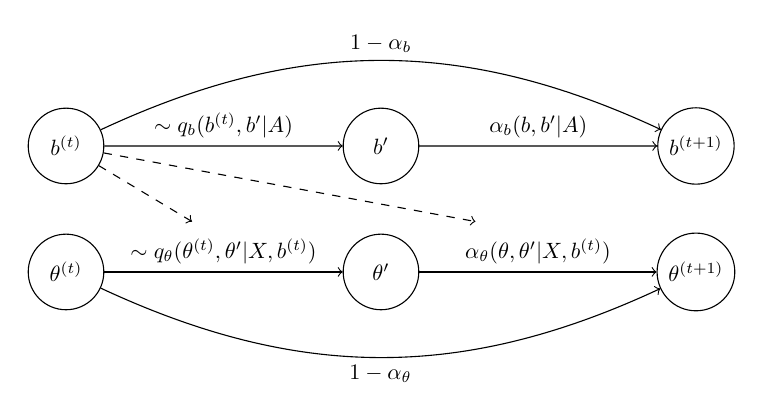
\begin{tikzpicture}[
		scale=0.8, every node/.style={transform shape},
		roundnode/.style={circle, draw=black, minimum size=12mm},
		squarednode/.style={rectangle, draw=black, minimum size=12mm}
		]
		% nodes
		\node[roundnode] (b0) at (0, 2) {$b^{(t)}$};
		\node[roundnode] (b1) at (5, 2) {$b'$};
		\node[roundnode] (b2) at (10, 2) {$b^{(t+1)}$};
		\node[roundnode] (t0) at (0, 0) {$\theta^{(t)}$};
		\node[roundnode] (t1) at (5, 0) {$\theta'$};
		\node[roundnode] (t2) at (10, 0) {$\theta^{(t+1)}$};
		
		% arrows
		\draw[->] (b0) to node[above] {$\sim q_b ( b^{(t)}, b' | A )$} (b1);
		\draw[->] (b1) to node[above] {$\alpha_b (b, b' | A )$} (b2);
		\draw[->] (b0) [out=25, in=155] to node[above] {$1-\alpha_b$} (b2);
		
		\draw[->] (t0) to node[above] {$\sim q_\theta(\theta^{(t)}, \theta' | X, b^{(t)})$} (t1);
		\draw[->] (t1) to node[above] {$\alpha_\theta (\theta, \theta' | X, b^{(t)})$} (t2);
		\draw[->] (t0) [out=-25, in=-155] to node[below] {$1-\alpha_\theta$} (t2);
		
		\draw[dashed, ->] (b0) to (2, 0.8);
		\draw[dashed, ->] (b0) to (6.5, 0.8);
		
	\end{tikzpicture}
	\caption{$\theta$-sample generation.}
	\label{fig:samp-sequence}
\end{figure}
 
Figure \ref{fig:samp-sequence} shows an overview of the proposed method, with $q$ and $\alpha$ denoting the MH proposal distribution and acceptance probability respectively.
Note the importance of the simplification in~(\ref{eqn:b-pseudo-prior}). 
As evaluating $p(b| X)$ does not depend on $X$, 
we do not need $X$ to sample $b$.
And on the other level, in order to obtain 
samples for $\theta$
we use only $b$ but not $A$, as $(\theta \indep A )| b$. 

\FloatBarrier
\subsection{Sampling block memberships}

To generate the required $b$-samples, we adopt the MCMC
procedure of
\cite{Peixoto-MCMC},
which relies on writing the posterior in the following form,
%
\begin{equation}
	p(b | A, X) \propto p(A | b, X) \cdot p(b | X) = \pi_b(b),
\end{equation}
%
where $\pi_b(\cdot)$ denotes the un-normalised target density.
Since we are using the microcanonical SBM formulation, there is only one 
value of $\psi$ that is compatible with the given $(A, b)$ pair;
recall the constraints in~(\ref{eqn:sbm-constraints}).
We denote this value $\psi^* = \{\psi_k^*, \psi_e^*\}$. Therefore, 
the summation over all $\psi$ needed to evaluate $p(A | b, X)$ reduces to just the single $\psi^*$ term:
$p(A | b, X) = \sum_{\psi} \nolimits p(A , \psi | b, X) = p(A, \psi^* | b, X)$.
In
this context, the microcanonical entropy of the configuration $b$
is,
%
\begin{equation}
	S(b) \coloneqq - \log \pi_b(b) = - \Big( \log p(A | b, \psi^*) + \log p(\psi^*, b | X) \Big),
	\label{eqn:dl-form}
\end{equation}
%
which can be thought of as the optimal
``description length'' of the graph. 
This expression will later be employed 
to help evaluate experimental results. 
The exact form of the proposal $q_b$ is explored thoroughly in
\cite{Peixoto-MCMC} and not repeated here. We use the \verb*|graph-tool| \cite{peixoto_graph-tool_2014}
library for Python, which implements this algorithm.
The only modification is in 
the prior $p(b)$ that we replace with $p(b|X)=B^{-N}$, 
which cancels out in the MH accept-reject step as it is independent of $b$.

\subsection{Sampling feature-to-block generator parameters}
\label{s:sfb}

The target distribution for the required $\theta$-samples 
is the posterior of $\theta$ given the values of the pair $(X, b)$. 
We write this as,
%
\begin{equation}
	\pi_\theta(\theta) \propto p(\theta | X, b) \propto p(b | X, \theta) p(\theta) \propto  \exp \left( - U(\theta) \right),
	\label{eq:U}
\end{equation}
%
where $U(\theta)$ denotes the negative log-posterior. Let $y_{ij} \coloneqq \one \left\{ b_i = j \right\}$ and $a_{ij} \coloneqq \phi_j(x_i; \theta)$. 
Discarding constant terms, $U(\theta)$ can be expressed as,
%
\begin{equation}
	U(\theta) = \left( \sum_{i \in [N]} \sum_{j \in [B]} y_{ij} \log \frac{1}{a_{ij}} \right)
	+ \frac{1}{2\sigma_\theta^2} \|\theta\|^2 = N \cdot \Lcal(\theta) + \frac{1}{2\sigma_\theta^2} \|\theta\|^2;
	\label{eqn:U-form}
\end{equation}
%
see Appendix \ref{appdx:form-U}. The function $U(\theta)$ is a typical objective function for neural network training. The first term $N \cdot \Lcal(\theta)$ is introduced by the likelihood and represents the cross-entropy between the graph-predicted and feature-predicted block memberships. 
The second term, introduced by the prior, brings a form of regularisation, guarding against over-fitting. In order to draw samples from the posterior 
$\pi_\theta \propto \exp(-U)$ we adopt the Metropolis-adjusted Langevin 
algorithm (MALA) \cite{mala-tweedie}, which uses $\nabla U$ to bias the 
proposal towards regions of higher density. Given the current 
sample $\theta$, a proposed 
new sample $\theta'$ is generated from,
%
\begin{equation*}
	\theta' \sim q_\theta\big(\theta, \theta'\big) 
	= \Gaussian \big( \theta' ; \theta - h \nabla U(\theta), 2h I \big),
\end{equation*}
%
where $\xi \sim \Gaussian(0, I)$ and $h$ is a step-size parameter 
which may vary with the sample index.
Without the injected noise term $\xi$, MALA is equivalent to gradient descent. We require $\xi$ to fully explore the parameter space. 
The term $\nabla U$ has an easy to compute analytic form (derived in Appendix \ref{appdx:form-U}).

\subsection{Sampling sequence}
\label{s:ss}

So far, each $\theta^{(t)}$ update has used its corresponding $b^{(t)}$ sample. This means the evaluation of $U^{(t)}$ and $\nabla U^{(t)}$ has high variance, leading to longer burn-in and possibly slower MCMC convergence. The only link between $b^{(t)}$ and $\theta^{(t)}$ is in the evaluation of $U^{(t)}$ and $\nabla U^{(t)}$ which depends only on the matrix $y^{(t)}$ with entries $y_{ij}^{(t)} \coloneqq \one\{b_i^{(t)} = j\}$. We would rather deal with the expectation of each $y_{ij}^{(t)}$:
%
\begin{equation}
	\Expect \left[ y_{ij}^{(t)} \right] = \Expect_{b^{(t)}} \left[ \one \left( b_{i}^{(t)} = j \right) \right]
	= p(b_i = j | A, X).
\end{equation}
%
An unbiased estimate for this can be obtained using 
the thinned $b$-samples after burn-in.
Let $\Tcal_b$  denote the retained set of indices 
for the $b$-samples and $\Tcal_\theta$ similarly for the $\theta$-chain. 
The unbiased estimate for $y_{ij}^{(t)}$ is then:
%
\begin{equation}
	\hat{y}_{ij} \coloneqq \frac{1}{|\Tcal_b|} \sum_{t \in \Tcal_b} y_{ij}^{(t)} = \frac{1}{|\Tcal_b|} \sum_{t \in \Tcal_b} \one\{b_i^{(t)} = j\}.
	\label{eqn:y-hat}
\end{equation}
%
The same matrix $\hat{y}$ is used in each $\theta^{(t)}$ update step.
This way, it is not necessary to run the $b$ and $\theta$ Markov chains 
concurrently. Instead, we run the $b$-chain to completion and use it 
to generate $\hat{y}$ also allowing us to vary the lengths of each.

\subsection{Dimensionality reduction}
\label{sec:dim-reduction}

The complexity of evaluating $U$ and $\nabla U$ is linear in 
the dimension of the feature space $D$,
so there is computational incentive to reduce $D$.
Given the samples $\left\{ \theta^{(t)} \right\}$, we can compute the empirical mean and standard deviation of each component of $\theta$. 
Switching to the matrix notation $W$ for $\theta$,
let:
%
\begin{equation}
	\hat{\mu}_{ij} \coloneqq \frac{1}{|\Tcal_\theta|} \sum_{t \in \Tcal_\theta} W_{ij}^{(t)} \qquad \textrm{and} \qquad
	\hat{\sigma}_{ij}^2 \coloneqq \frac{1}{|\Tcal_\theta|} \sum_{t \in \Tcal_\theta} \left( W_{ij}^{(t)} - \hat{\mu}_{ij} \right)^2.
\end{equation}
%
A simple heuristic to discard the least important features requires specifying a cutoff $c > 0$ and a multiplier $k > 0$. We define the function $\Fcal_i(j)$ 
as in~(\ref{eqn:fij}) and only keep features with indices $d \in \Dcal'$, where $\Dcal'$ is given in~(\ref{eqn:kept-feature-set}).
%
\begin{align}
	\Fcal_i(j) &\coloneqq (\hat{\mu}_{ij} - k \hat{\sigma}_{ij}, \hat{\mu}_{ij} + k \hat{\sigma}_{ij}) \cap (-c, +c),
	\label{eqn:fij} \\
	\Dcal' &\coloneqq \left\{ j \in [D] : \exists i \in [B] \textrm{ s.t. }  \Fcal_i(j) = \emptyset \right\}.
	\label{eqn:kept-feature-set}
\end{align}
%
Intuitively, this means discarding any feature $j$ for which 
$(\hat{\mu}_{ij} - k\hat{\sigma}_{ij}, \hat{\mu}_{ij} + k \hat{\sigma}_{ij})$ overlaps with
$(-c, c)$ for all $i$. If we were to use the Laplace approximation for the posterior $p(W_{ij} | A, X) \approx \Gaussian(W_{ij}; \hat{\mu}_{ij}, \hat{\sigma}_{ij}^2)$, then this would be analogous to a hypothesis test on the magnitude of $W_{ij}$ compared to $c$ with multiplier $k$ in~(\ref{eqn:fij}) determining the degree of significance of the result. Conversely, if we want to fix the number of dimensions in our reduced feature set $|\Dcal'|=D'$, the problem then becomes finding the largest value of $c$ such that $|\Dcal'|=D'$ given $k=k_0$:
%
\begin{equation}
	c^* = \argmax \{c>0\; : \;|\Dcal'| = D', k=k_0\}.
	\label{eqn:c-star}
\end{equation}


	\section{Experiments}

We apply the developed methods to a variety of datasets, to show the power of the method across different scenarios. We choose datasets to span a range of node counts $N$, edge counts $E$ and feature space dimension $D$.

\begin{itemize}
	\item \textbf{Political books} \cite{polbooks} ($N=105, E=441, D=3$) - network of Amazon book sales about U.S. politics, published close to the presidential election in 2004. Two books are connected if they were frequently co-purchased by the same customer. Vertex features encode the broad political affiliation of the author (liberal, conservative or neutral).
		
	\item \textbf{Primary school dynamic contacts} \cite{schools} ($N=238, E=5539, D=13$) - network of face-to-face contacts amongst students and teachers at a primary school in Lyon, France. Two nodes are connected if the two parties shared a face-to-face interaction over the course of the day. Vertex features include class membership, gender and whether or not the individual is a teacher or pupil. These data were collected on consecutive days in October 2009. We choose to analyse just the second day.
	
	\item \textbf{Facebook egonet} \cite{fb-snap} ($N=747, E=30025, D=480$) - an assortment of Facebook egonets. These are networks of a particular user's friends list and all the connections within that. Vertex features are extracted from each user's profile and are fully anonymized. We focus on the egonet with id 1912.
	
%	\item \textbf{Maier Facebook Egonet} \cite{FB-Maier}  ($N=349, E=2336, D=32$) - egonet of the author's Facebook friends list. Each vertex has been manually labelled with a variety of features describing their relationship to the author. For our purposes we remove all nodes of degree 1 (those that are only connected to the egonode) as these cannot be said to be part of any community present in the graph.
%		
%	\item \textbf{Law firm} \cite{LawFirm} - a network of relationships between members of a law firm. Each relationship is categorised according to type: coworkers, friends or advice.
%	
%	\item \textbf{Twitch users} \cite{twitch} - a network of user-user friendships on the streaming service Twitch. Vertex labels are extracted according to video-games played, location and streaming habits. This dataset is also broken down into disjoint networks according to language. We only consider the English users with is a subnet with $N=7126$ vertices and $E=35324$ edges).

\end{itemize}

We require metrics to assess the relative model evidence for the FFBM. This can be split into two separate components: the microcanonical SBM fit (concerned with the $b$-samples) and the fit of the feature-to-block generator (concerned with the $\theta$-samples). For each of these we can evaluate the mean of the unnormalised log-target of each Markov chain.
%
\begin{equation}
	\bar{S}_b \coloneqq \frac{1}{T_b} \sum_{t=1}^{T_b} S \left( b^{(t)} \right) \qquad \textrm{and} \qquad
	\bar{U}_\theta \coloneqq \frac{1}{T_\theta} \sum_{t=1}^{T_\theta} U \left( \theta^{(t)} \right)
\end{equation}
%
The lower these quantities, the better the fit of each stage of the model. To allow for rough comparison between datasets, we divide these quantities by the number of vertices in the graph $N$. Table \ref{tab:results} summarises the results for each experiment.

\begin{table}[!h]
	\centering
	\caption{FFBM fit for the datasets}
	\label{tab:results}
	\begin{tabular}{c|ccc|c|cc}
		Dataset & $N$ & $E$ & $D$ & $B$ & $\bar{S}_b /N$ & $\bar{U}_\theta /N$ \\ \hline
		Political books & 105  & 441 & 3 & 3 & 11.7 & 0.707 \\
		Primary school & 238 & 5539 & 13 &  10 & 45.9  & 1.61 \\
		FB egonet & 747 & 30025 & 480 & 10  & 66.9 & 7.47
	\end{tabular}
\end{table}

\FloatBarrier
\subsection{Political books}

This dataset was collected by \citet{polbooks}. We wish to determine whether political affiliation is a good predictor of the overall network structure. We choose to partition the network into $B=3$ communities as we only have this many distinct values for political affiliation (conservative, liberal or neutral). The inferred block memberships are given in figure \ref{fig:books-graph}. We sample the block-generator parameters and plot the emprical mean and standard deviation of each sample on figure \ref{fig:book-null}.
%
\begin{figure}[!h]
	\centering
	\begin{subfigure}{0.3\linewidth}
		\centering
		\includegraphics[width=\linewidth]{polbooks-graph.png}
		\fbox{\includegraphics[width=0.4\linewidth]{3-legend.png}}
		\caption{Sampled block memberships $\hat{Y}$}
		\label{fig:books-graph}
	\end{subfigure}
	\hfill
	\begin{subfigure}{0.5\linewidth}
		\centering
		\includegraphics[width=\linewidth]{polbooks-null.png}
		\caption{Feature weights}
		\label{fig:book-null}
	\end{subfigure}
	\caption{Political books network \cite{polbooks}}
\end{figure}
%
Indeed, for all 3 blocks, each has a distinct political affiliation as its highest magnitude component. This is strong evidence that political affiliation is indeed the axis which best predicts the 3-way natural partition of the graph into blocks. Nevertheless, for block index 1, although \verb*|neutral| is the best predictor of the ones we have available, the value is not particularly extreme. Perhaps, there is an unobserved feature that places a book into this block. Indeed, block-0 is more of a centre-right block than true centre.

\FloatBarrier
\subsection{Primary school dynamic contacts}

These data were originally collected by \citet{schools} to quantify the transmission opportunities for respiratory infections. However, we seek to ask which vertex features best describe how people interact with one another in a primary school context. The only vertex features we have available are school-class (one of 10 values - 2 per year group), gender and a distinction between teachers and pupils.

We must first choose the number of blocks $B$ to define the coarseness of our analysis. A total of 10 school-classes would suggest that $B=10$ is a natural starting point. We visualise the inferred block memberships in figure \ref{fig:school-graph}.
%
\begin{figure}[!h]
	\centering
	\begin{subfigure}{0.45\linewidth}
		\centering
		\includegraphics[width=\linewidth]{school-graph.png}
		\fbox{\includegraphics[width=0.5\linewidth]{10-legend.png}}
		\caption{Sampled block memberships $\hat{Y}$}
		\label{fig:school-graph}
	\end{subfigure}
	\hfill
	\begin{subfigure}{0.45\linewidth}
		\centering
		\includegraphics[width=\linewidth]{school-null.png}
		\caption{Reduced dimension feature weights}
		\label{fig:school-null}
	\end{subfigure}
	\caption{Primary school dynamic contacts network \cite{schools}}
\end{figure}

As before, we proceed to sample the block-generator parameters $\theta$ and employ the dimensionality reduction heuristic defined in section \ref{sec:dim-reduction} with null threshold $c=1$ and standard deviation multiplier $k=1$. We then plot the weights for the features that survive the discard step in figure \ref{sec:dim-reduction}. Immediately, we see that only the pupils' class memberships have survived (1A-5B); gender and teacher/student status have been discarded meaning that these are not good predictors of overall macro-structure.

The vast majority of blocks are composed of a single class. However, some blocks have 2 comparably good classes as their predictor. For example, blocks 2 and 4 contain classes 4A and 4B as their 2 best predictors. This suggests that the social divide between classes is less pronounced for pupils in year 4 but there is nonetheless an unobserved variable that splits year 4 into 2 communities. The most surprising block is number 5 - which has comparable weightings for classes 5A and 1B. Perhaps there was a joint event between those two classes on the day the data were collected.

\subsection{Facebook egonet}

This dataset was chosen to showcase the power of the dimensionality reduction technique as the feature-space has high dimension ($D=480$). We sample the $b$-chain specifying $B=10$ total blocks and use this to construct the $\theta$-samples as before. 

We apply the dimensionality reduction heuristic outlined in section \ref{sec:dim-reduction}, choosing $k=1$ and $c=0.8$. This leads to a reduced dimension $D'=13$. These parameter values are plotted on figure \ref{fig:fb-null}. The features that remain are those that best explain the high-level community structure. More so than language, gender or surname - the school\footnote{This includes higher education institutes} you attend is the best explanatory variable for how the observed network's communities are partitioned at the highest level. 
%
\begin{figure}[!h]
	\centering
	\begin{subfigure}{0.45\linewidth}
		\centering
		\includegraphics[width=\linewidth]{fb-graph.png}
		\fbox{\includegraphics[width=0.3\linewidth]{10-legend.png}}
		\caption{Sampled block memberships $\hat{Y}$}
		\label{fig:fb-graph}
	\end{subfigure}
	\hfill
	\begin{subfigure}{0.45\linewidth}
		\centering
		\includegraphics[width=\linewidth]{fb-null.png}
		\caption{Reduced dimension feature weights}
		\label{fig:fb-null}
	\end{subfigure}
	\caption{Facebook egonet id 1912 \cite{fb-snap}}
\end{figure}

Nevertheless, this example also highlights a weakness of the method for high-dimensional feature spaces. When the feature dimension is very large, it becomes increasingly likely that a particular feature may uniquely identify a small set of nodes. If these nodes are all part of the same community then the classifier will overfit for that particular parameter. The regularisation term imposed by the prior goes some way to alleviating this problem but we see in figure \ref{fig:fb-null} that the feature \verb*|birthday-5| has a very high weight as it relates to block 0. It might be possible to shift the feature values such that they take values in $\{-1, 1\}$ rather than $\{0, 1\}$ but this approach falls down when input features are mutually correlated. Indeed, for features with discrete values such as the class memberships (1A, 1B, 2A \dots 5B) it is preferred to keep $x_i \in \{0, 1\}^D$ as then each block can be readily accept more than one mutually exclusive feature-group (i.e. two school-classes are part of the same block).


	%\section{Extensions}

The greatest limitation of the current FFBM formulation is that it can only explain structure at the macro-scale. In other words, we cannot explain structure within each detected block. Future work will benefit from extending the FFBM to be hierarchical in nature. This would be a relatively natural extension. Indeed, the SBM has already been extended to a hierarchical form, often called the nested SBM \cite{SBM-hierarchical}. The idea is to divide each block into sub-blocks and so on recursively until a specified depth is reached. The full block membership for a particular vertex now encodes the memberships at all levels of the hierarchy.

The necessary modification of the feature-to-block generator is also rather natural. Given the nested SBM, we would have a hierarchy of generators, each generating a block membership at a particular level of the hierarchy. Nevertheless, this does pose some practical issues for scalability; supposing we have $L$ levels in our hierarchy and each divides the parent block into $B$ sub-blocks, then the number of distinct generators necessary scales as $O(B^L)$. To avoid exponential growth in the number of model parameters, we could apply some form of dimensionality reduction as we descend the layers so that each generator is only given relevant features as input.
	\section{Conclusion}
\label{sec:conclusion}

An efficient MCMC algorithm 
is developed for sampling 
from the posterior distribution of
the relevant parameters in the FFBM;
the main idea is to divide up the graph into 
its most natural partition under the associated
parameter values, and then to determine whether 
the vertex features can accurately explain the partition. 
Through several applications on empirical
network data, this approach 
is shown to be effective at extracting and describing 
the most natural communities in a labelled network. 
Nevertheless, it
can only currently explain the structure at the macroscopic
scale. Future work will benefit from extending 
the FFBM to a further hierarchical model,
so that
the structure of the network 
can be explained at all scales of interest.



	
	\appendix
	%\section{Appendix: Additional material}

\subsection{SBM likelihood and prior}
\label{appdx:sbm}

For reference, we provide the likelihood and priors for the microcanonical SBM proposed by \citet{Peixoto-Bayesian-Microcanonical}. We have that the graph $A$ is drawn from the SBM:
%
\begin{equation}
	A \sim \textrm{DC-SBM}_{\textrm{MC}}(b, e, k)
\end{equation}
%
With edges placed uniformly at random but respecting the constraints imposed by $b, e$ and $k$. The likelihood calculation for $p(A|k, e, b)$ then reduces to a case of counting configurations that yield the same adjacency matrix, $\Xi (A)$, and dividing by the total number of configurations possible, $\Omega(e)$. This is why this formulation is given the microcanonical moniker. If we consider the half-edges to be distinguishable for a moment, the total number of configurations that satisfy the $e$ constraint is:
%
\begin{equation}
	\Omega(e) = \frac{\prod_{r} e_r !}{\prod_{r,s : r < s} e_{rs}! \cdot \prod_{r} e_{rr}!!}
\end{equation}
%
Where $e_r \coloneqq \sum_{s} e_{rs}$ and $(2m)!! \coloneqq 2^m m!$. Nevertheless, a great number of these configurations yield the same graph $A$. We denote the number of configurations that yield the adjacency matrix $A$ with $\Xi(A)$, which can be computed as:
%
\begin{equation}
	\Xi(A) \coloneqq \frac{\prod_i k_i !}{\prod_{i,j : i < j} A_{ij} ! \prod_i A_{ii} !! }
\end{equation}
%
Note the similarity between the forms of $\Omega(e)$ and $\Xi(A)$ as $e$ is effectively the adjacency matrix of the block-graph. With these defined we can write the overall likelihood:
%
\begin{equation}
	p(A|k,e,b) = \frac{\Xi(A)}{\Omega(e)}
\end{equation}
%
Obviously, this form is only defined if $A$ respects the constraints imposed by $(k,e,b)$ else the likelihood is 0. With the likelihood defined, we move on to the prior. As discussed in the main text, the block membership vector $b$ is an intermediate variable in the FFBM and not a parameter so we are not free to choose a prior for it. Nevertheless, we can borrow the conditional prior proposed by \citet{Peixoto-Bayesian-Microcanonical} for the other parameters to give:
%
\begin{equation}
	p(e, k | b) = p(e | b) p(k| e, b) = \left[ \specialchoose{ \specialchoose{B}{2} }{ E} \right]^{-1} 
	\cdot \left[ \prod_r \frac{\prod_j \eta_j^r !}{n_r! q(e_r, n_r)} \right]
\end{equation}
%
Where $\specialchoose{n}{m}$ is shorthand for $\binom{n+m-1}{m} = \frac{(n+m-1)!}{(n-1)!(m)!}$ which can be thought of as the total number of distinct histograms with $n$ bins under the constraint they sum to $m$. $E = \frac{1}{2} \sum_{r,s} e_{rs}$ is the total number of edges in the graph. Importantly, $E$ is not allowed to vary and so $p(e|b)$ is uniform with respect to $e$. The variable $\eta_j^r$ is introduced to denote the number of vertices in block $r$ that have degree $j$. Formally, $\eta_j^r \coloneqq \sum_{i} \one\left\{b_i = r \right\} \one \left\{k_i = j \right\}$. Furthermore, $q(m, n)$ is the number of different histograms with at most $n$ non-zero bins that sum to $m$. $q(m, n)$ is related to but different from $\specialchoose{n}{m}$. Recall that $e_r \coloneqq \sum_{s} e_{rs}$ is the total number of half edges in block r and $n_r \coloneqq \sum_{i} \one\{b_i = r\}$ is the number of vertices assigned to block $r$. 

The form of these priors were chosen carefully by \citet{Peixoto-Bayesian-Microcanonical} to more closely match the structure of empirical networks than simple uniform priors. We do not repeat his arguments here.

\subsection{Choosing the MALA step-size}
\label{appdx:step-size}

For sampling from the $\theta$-chain of the block membership generator parameters, we employ the Metropolis Adjusted Langevin Algorithm (MALA). At iteration $t$, the proposed sample is generated by:
%
\begin{equation}
	\theta' = \theta^{(t)} - h_t \nabla U(\theta^{(t)}) + \sqrt{2h_t} \cdot \xi
\end{equation}
%
There are two competing objectives when choosing the step-size $h_t$. On the one hand, we want the step-size to be large so that we arrive at a high density region quickly. However, too large a step-size will lead to a lower acceptance ratio and thus inefficient sampling. A solution to this problem would be to slowly decrease the step-size with $t$ - often called simulated annealing. Therefore, we still have a short burn-in time but will not bounce around the mode for large $t$. As well as the trivial constraint for $h_t$ to be strictly positive, we introduce two further constraints as outlined by \citet{Bayesian-SGLD}:
%
\begin{equation}
	\sum_{t=1}^{\infty} h_t = \infty \qquad \textrm{and} \qquad
	\sum_{t=1}^{\infty} h_t^2 < \infty
	\label{eqn:h-constraints}
\end{equation}
%
The first constraint ensures that we can cover sufficient distance to arrive at any arbitrary point in our domain, no matter the starting point. The second constraint ensures that once we converge to the mode we will stay there, rather than simply bouncing around it. \citet{Bayesian-SGLD} propose the following form for a polynomially decaying step-size which we adopt:
%
\begin{equation}
	h_t = \alpha(\beta + t)^{-\gamma}
\end{equation}
%
Where $\alpha, \beta, \gamma$ are hyper-parameters to be chosen. We require $\alpha,\beta > 0$ and $\gamma \in (0.5, 1]$ to satisfy equation \ref{eqn:h-constraints}. To reduce the number of hyperparameters we set these to have values given by the equations in \ref{eqn:step-size-params}.
%
\begin{equation}
	\alpha = \frac{250 \cdot s}{N} \qquad \beta = 1000 \qquad \gamma = 0.8
	\label{eqn:step-size-params}
\end{equation}
%
Where $N$ is the number of data-points we are considering and now $s$ is the only free variable which we call the step-size scaling. For approximate methods, we can choose to bypass the MH accept-reject entirely to speed up computation. If this is done, the algorithm is instead called stochastic gradient Langevin diffusion (SGLD) \cite{Bayesian-SGLD}. This speeds up computation at the expense of the exactness of the method. Indeed, it relies on the fact that as the step-size is annealed to 0, the acceptance probability is close 1.

Nevertheless, to choose the value of $s$ we must quantify the trade-off between acceptance ratio and burn-in time. We do this by way of an example with the primary school dataset \cite{schools}. We run the $b$-chain for $T_b = 1,000$ iterations and subsample such that $\Tcal_b$ is computed with $\kappa_b=0.2$ and $\lambda_b=5$. We then use this to run the $\theta$-chain for $T_\theta = 10,000$ iterations. The acceptance ratio -- which we denote $r_\alpha$ -- is easy enough to compute as simply the fraction of proposed moves which we accept. However, to quantify burn-in time we must use a different metric. We can plot the mean of the objective function averaged over all samples as a proxy for burn-in time:
%
\begin{equation}
	\bar{U} \coloneqq \frac{1}{T_\theta} \sum_{t \in [T_\theta]} U\left( \theta^{(t)} \right)
\end{equation}
%
As the chain will equilibrate in the vicinity of a minima in $U(\theta)$, the average over all samples is a rough indicator of the speed of burn-in. This assumes that the random starting point has high $U(\theta)$. This assumption holds as the domain of $\theta$ is a high dimensional space so we are unlikely to get a low $U(\theta)$ simply from a lucky guess. The higher the value of $\bar{U}$, the longer we infer the chain took to burn in and reach equilibrium. We plot the acceptance ratio $r_\alpha$ and average objective $\bar{U}$ for $10$ values of the step-size multiplier $s$ logarithmically spaced in the range $(10^{-2}, 10^1)$ on figure \ref{fig:step-size-tradeoff}.
%
\begin{figure}[!h]
	\centering
	\includegraphics[width=0.6\linewidth]{step-size-tradeoff}
	\caption{Primary school dataset \cite{schools} illustration of step-size tradeoff}
	\label{fig:step-size-tradeoff}
\end{figure}

We see immediately that acceptance ratio $r_\alpha$ steadily decreases with $s$. This is expected as it is unlikely we stay in a high density region of our target distribution if we are making very large steps each time. A low acceptance ratio leads to wasted samples and this inefficiency is obviously undesirable. Indeed, figure \ref{fig:step-size-tradeoff} suggests that a low step-size $s$ yields high acceptance probability thus justifying the approximation used in SGLD.

Nevertheless, $\bar{U}$ decreases with $s$ indicating shorter burn-in times for larger step-sizes. However, this effect plateaus for $s>0.2$ for this particular dataset. Therefore, we choose $s=0.2$ as our step-size multiplier for the primary school datasets as this yields the best trade-off between $r_\alpha$ and $\bar{U}$. Indeed, the acceptance ratio is still high for $r_\alpha \approx 0.8$ for $s=0.2$. The step-sizes for the other datasets were chosen following the same argument but we do not repeat the process here.

\FloatBarrier
\subsection{Burn-in and thinning}
\label{appdx:burn-in-thinning}

As with any MCMC method, we must deal with the issues presented by burn-in and thinning. We have introduced the notation $\Tcal_b$ and $\Tcal_\theta$ to denote the set of samples we keep from the $b$ and $\theta$ chains respectively. Note that we generate $T_b$ and $T_\theta$ samples total. The burn-in period refers to the time taken for the Markov Chain to converge to the stationary distribution. Sample thinning is necessary to ensure that neighbouring samples satisfy independence. However, as we do not leverage the independence property this is less important in our analysis. We can write the general set $\Tcal_\star$ as:
%
\begin{equation}
	\Tcal_\star = \{T_\star \kappa_\star + i \lambda_\star :  
	0 \leq i \leq \lfloor T_\star(1 - \kappa_\star) / \lambda_\star \rfloor \}
\end{equation}
%
Where the parameter $\kappa_\star \in (0, 1)$ controls our burn-in and $\lambda_\star$ controls our thinning. $\kappa_\star$ can be determined by plotting the log-target (either $S(b^{(t)})$ or $U(\theta^{(t)})$ with respect to the epoch $t$. $\kappa_\star$ is then chosen to encompass the region where the log-target has roughly equilibrated. As we do not leverage sample independence $\lambda_\star$ can be chosen less rigorously. We often just use $\lambda_b=5$ and $\lambda_\theta = 10$.

By way of illustration, we can consider the primary school dataset \cite{schools}. We plot the normalised objective function $U\left( \theta^{(t)} \right) / N$ with respect to MALA iteration on figure \ref{fig:school-U-orginal}. We see that the chain converges to the modal neighbourhood quickly (within about 2000 iterations of a total 10,000). Nevertheless, we pick $\kappa_\theta=0.4 > 0.2$ just to be on the safe-side. $\lambda_\theta=10$ is chosen somewhat arbitrarily as we do not require neighbouring samples to be independent. Nevertheless, this thinning does speed up computation of quantities that require an average over all the retained samples -- as $|\Tcal_\theta| < T_\theta$.
%
\begin{figure}[!h]
	\centering
	\begin{subfigure}[t]{0.4\linewidth}
		\centering
		\includegraphics[width=\linewidth]{school-U-original.png}
		\caption{Original samples $t \in [T_\theta]$}
		\label{fig:school-U-orginal}
	\end{subfigure}
	\begin{subfigure}[t]{0.4\linewidth}
		\centering
		\includegraphics[width=\linewidth]{school-U-thinned.png}
		\caption{Thinned samples $t \in \Tcal_\theta$ indexed by $i$}
		\label{fig:school-U-thinned}
	\end{subfigure}
	\hspace{1cm}
	\caption{Primary school dataset normalised objective function against sample index}
\end{figure}

We see on figure \ref{fig:school-U-thinned} that $U(\theta^{(i)})$ does bounce around a small amount. This is to be expected we are sampling from the posterior rather than converging to the MAP. There does appear to be variation over a long time-scale but we can live with this as we do not require sample independence.
\FloatBarrier
\subsection{Initializing the b-chain}

For the purposes of our model (the FFBM), the number of blocks $B$ is a constant which must be specified by the data scientist. We could however, allow our choice of $B$ to be influenced by the observed data. This places us in the domain of empirical Bayes, which must be negotiated carefully. Prior beliefs must be determined a priori else they are not prior. However, as the number of blocks only specifies the coarseness of the analysis, it is fine to allow it to vary. Indeed, \citet{peixoto-determine-B} shows that for a fixed average degree the maximum number of detectable blocks scales as $O(\sqrt{N})$ where $N$ is the number of vertices.

If we allow $B$ to vary in the $b$-chain (i.e. new blocks can be created and we permit empty blocks) then it can be run  until a minimum description length (MDL) solution is reached. We take the number of non-empty blocks at the MDL solution to be our fixed block number $B$ for subsequent analysis. Indeed, it is prudent to start our $b$-chain at this MDL solution as then we can burn-in time is greatly reduced.

\subsection{Dimensionality discussion}
\label{appdx:dimension}

There is a challenge when dealing with vertex-features. Many vertex feature often take only one of several discrete values within a set. For example, with the primary school dataset \cite{schools}, a pupil's school-class can take one of 10 values from \{"1A", "1B", "2A", "2B" \dots "5A", "5B"\}.

It is not immediately obvious how to encode this for the feature-to-block classifier. Although this is technically only a single dimension, we choose to expand the data into a set of 10 binary feature flags $\in \Xcal = \{0, 1\}$. Although only one flag will be set at a time it is the simplest method for representing discrete-valued data. The reason we choose $\Xcal=\{0, 1\}$ and not $\Xcal = \{-1, 1\}$ is that the former allows for simpler analysis of the resulting weight values; when a feature $d$ is switched off then $x_{d}=0$ given $\Xcal = \{0, 1\}$, and the feature has no impact on the softmax layer.

It is more intuitive to only model positive relationships. In other words, we prefer to say that this block is comprised of the vertices with feature $d$ turned on rather than this block contains the vertices with feature $d$ switched off. To make this explicit, say we have a feature encoding a pupil's gender: \{"male", "female"\}, we represent this as 2 binary feature flags "male": \{0, 1\} and "female": \{0, 1\}. This approach may seem inefficient but it is vital to ensure we can interpret the resulting parameter distributions.

Nevertheless, this dimensionality expansion means that we cannot include a bias term in our classifier as then the MAP solution is less peaked and our $\theta$-samples will have higher variance. To illustrate this point we need only look at the form of the soft-max classifier with bias vector $\beta$, operating on a vector $x$ which only has one non-zero entry $x_d=1$. Component $j$ of the output is given by:
%
\begin{equation}
	\phi_j(x) = \frac{\exp(w_j^T x + \beta_j)}{\sum_{k \in [B]} \exp(w_k^T x + \beta_k)} = 
	\frac{\exp(w_{jd} + \beta_j)}{\sum_{k \in [B]} \exp({w_{kd} + \beta_k})}
	\label{eqn:softmax-bias}
\end{equation}
%
The term $w_{kd} + \beta_k$ is effectively the new weight for component $k$ as this term always appears together. The bias term $\beta_k$ is an unnecessary extra degree of freedom. To illustrate this point, we set $\beta_k=\beta_0 \forall j$. If this is the case then equation \ref{eqn:softmax-bias} can be simplified to:
%
\begin{equation}
	\phi_j(x) = \frac{\exp(\beta_0) \cdot \exp(w_{jd})}{\sum_{k \in [B]} \exp(\beta_0) \cdot \exp(w_{kd})}
	= \frac{\exp(w_{jd})}{\sum_{k \in [B]} \exp(w_{kd})}
\end{equation}
%
This expression is independent of $\beta_0$ and so it is free to vary. This is not the whole picture as we also have the prior which introduces a regularisation term which favours weights closer to 0. Nevertheless, for mutually exclusive binary feature flags, the bias term does not add to the expressiveness of the model and only serves to complicate analysis. We therefore remove the bias term from the Softmax classifier. Even for data comprised of several such features (e.g. school class and gender) we prefer to discard the bias term. The bias term only serves to decrease the loss function by leveraging information about the size of each detected block and not feature information. We do not wish to be overly confident in our block predictions when such predictions are influenced by block size and not feature information. Indeed, the approach was initially developed with a bias term but we found its removal yielded more reliable and reproducible results.
	\section{Appendix: Derivations}

\subsection{Derivation of conditional block distribution given feature matrix}
\label{appdx:b|x}

We wish to determine the form of $p(b| X)$. This can be done by integrating over the joint probability with respect to $\theta$.
%
\begin{align*}
	p(b | X) &= \int p(b , \theta| X, \theta) d\theta = \int p(b | X, \theta) p(\theta | X) d\theta \\
	&=\int p(b | X, \theta) p(\theta) d\theta = \int \prod_{i \in [N] } \phi_{b_i}(x_i; \theta) p(\theta) d\theta \\
	&= \prod_{i \in [N]} \int \frac{\exp(w_{b_i}^T \tilde{x}_i) \prod_{j \in [B]} \Gaussian(w_j; 0, \sigma_\theta^2 I)}{\sum_{k \in [B]} \exp(w_{k}^T \tilde{x}_i)} dw_{1:B}
\end{align*}
%
We note that $b_i \in [B]$ and so the integral's value is unchanged with respect to $b_i$. The integrand has the same form no matter which value $b_i$ takes as the prior is the same for each $w_j$. As such the integral can only be a function of at most $\tilde{x}_i$ and $\sigma_\theta^2$ as it is symmetric with respect to $b_i$ and all the various $w_j$ are integrated out as they are dummy variables. Therefore, denoting the integral by the (unknown) function $f(\tilde{x}_i, \sigma_\theta^2)$, we write $p(b| X)$ as follows:
%
\begin{align*}
	p(b | X) &= \prod_{i=1}^{N} f(\tilde{x}_i, \sigma_\theta^2) = \textrm{const w.r.t } b = c
\end{align*}
%
As this is a constant with respect to $b$ we conclude that $p(b | X)$ must be a uniform distribution. $\nicefrac{1}{c}$ is simply the size of the set of values that $b$ can take. We know $b_i \in [B]$. Therefore, $b \in [B]^N$ and $|[B]^N| = B^N = \nicefrac{1}{c}$. Putting this all together we conclude that:
%
\begin{equation}
	p(b | X) = B^{-N}
\end{equation}

\subsection{Derivation of U form}
\label{appdx:form-U}

The invariant distribution we wish to target for the $\theta$ samples is the posterior of $\theta$ given the values of the pair $(X, b)$. We write this as follows:
%
\begin{align}
	\pi_\theta(\theta) &\propto p(\theta | X, b) \propto p(b | X, \theta) p(\theta) \propto  \exp \left( - U(\theta) \right) \\
	\therefore U(\theta) &= - \left( \log p(b | X, \theta) + \log p(\theta) \right) + \textrm{const}
\end{align}
%
Where we have introduced $U(\theta)$ equal to the negative log posterior. Each of the constituent terms of $U(\theta)$ are easily computed (equation \ref{eqn:U-constituent-terms}) by defining $y_{ij} \coloneqq \one \left\{ b_i = j \right\}$ and $a_{ij} \coloneqq \phi_j(x_i; \theta)$.
%
\begin{equation}
	\log p(b | X, \theta) = \sum_{i \in [N]} \sum_{j \in [B]} y_{ij} \log a_{ij}  \quad \textrm{and} \quad
	\log p(\theta) = -\frac{(D+1)(B)}{2} \log 2\pi - \frac{1}{2 \sigma_\theta^2} || \theta ||^2
	\label{eqn:U-constituent-terms}
\end{equation}
%
Discarding constant terms, we write $U(\theta)$ as in equation \ref{eqn:U-form-appdx-0}. Note that $||\theta||^2 = \sum_{i} \theta_{i}^2 = \sum_{j=1}^{B} ||w_j||^2$ is the Euclidean norm of the vector of parameters $\theta$.
%
\begin{equation}
	U(\theta) = \left( \sum_{i=1}^{N} \sum_{j=1}^{B} y_{ij} \log \frac{1}{a_{ij}} \right)
	+ \frac{1}{2\sigma_\theta^2} ||\theta||^2 = N \cdot \Lcal(\theta) + \frac{1}{2\sigma_\theta^2} ||\theta||^2
	\label{eqn:U-form-appdx-0}
\end{equation}
%

\subsection{Derivation of U gradient with respect to feature parameters}
\label{appdx:gradu}
The goal is to determine $\nabla U(\theta)$, the gradient of the negative log posterior with respect to the parameters. We repeat the form of $U(\theta)$ in equation \ref{eqn:U-form-appdx}.
%
\begin{equation}
	U(\theta) = \left( \sum_{i \in [N]} \sum_{j \in [B]} y_{ij} \log \frac{1}{a_{ij}} \right)
	+ \frac{1}{2\sigma_\theta^2} ||\theta||^2
	\label{eqn:U-form-appdx}
\end{equation}
%
Where $y_{ij}$ is independent of $\theta$ and $a_{ij}$ is the output from the softmax layer, with form as given in equation \ref{eqn:a-ij}.
%
\begin{equation}
	a_{ij} \coloneqq \phi_{j} (x_i; \theta) = \frac{\exp(w_j^T \tilde{x}_i)}{\sum_{r \in [B]} \exp(w_r^T \tilde{x}_i)}
	\label{eqn:a-ij} 
\end{equation}
%
We note that $\theta = \{w_k\}_{k=1}^B$, and as such we can write this in vector form $\theta = \left[w_1^T, w_2^T \dots w_B^T  \right]^T$. Therefore, $\nabla U(\theta) = \left[\nicefrac{\partial U}{\partial w_1}^T,\nicefrac{\partial U}{\partial w_2}^T \dots \nicefrac{\partial U}{\partial w_B}^T  \right]^T$; to compute $\nabla U(\theta)$ it suffices to find the form of $\nicefrac{\partial U}{\partial w_k}$ with respect to a general $k$.

To this end, we must first find partial derivatives of $a_{ij}$ and $||\theta||$ with respect to $w_k$. Starting with $a_{ij}$:
%
\begin{align}
	\frac{\partial a_{ij}}{\partial w_k} &= \frac
	{\tilde{x}_i \exp(w_j^T \tilde{x}_i) \delta_{jk} \cdot \sum_{r \in [B]} \exp(w_r^T \tilde{x}_i) 
		- 
		\exp(w_j^T \tilde{x}_i) \cdot \tilde{x}_i \exp(w_k^T \tilde{x}_i)}
	{\left( \sum_{r \in [B]} \exp(w_r^T \tilde{x}_i) \right)^2} \nonumber \\
	&= \tilde{x}_i \left( a_{ij} \delta_{jk} - a_{ij}a_{ik} \right) 
\end{align}
%
Where $\delta_{jk} \coloneqq \one \left\{ j = k \right\}$. Now moving onto the derivative of $||\theta||^2$:
%
\begin{equation}
	\frac{ \partial}{\partial w_k} ||\theta||^2 = \frac{\partial}{\partial w_k} \left( \sum_{r \in [B]} ||w_r||^2 \right) = 2w_k
\end{equation}
%
We are ready to put this all together, to find the partial derivative of $U(\theta)$ with respect to each $w_k$:
\begin{align}
	\frac{\partial U}{\partial w_k} &= 
	\sum_{i=1}^{N} \sum_{j=1}^{B} y_{ij} 
	\left( \frac{-\tilde{x}_i}{a_{ij}} \left( a_{ij} \delta_{jk} - a_{ij} a_{ik} \right) \right)
	+ \frac{w_k}{\sigma_\theta^2} \nonumber \\
	&=  - \left( \sum_{i=1}^{N} \tilde{x}_i \left( y_{ik} - a_{ik} \sum_{j=1}^{B} y_{ij} \right)
	- \frac{w_k}{\sigma_\theta^2} \right) \nonumber \\
	&= - \left( \sum_{i=1}^{N} \Big\{ \tilde{x}_i (y_{ik} - a_{ik}) \Big\} - \frac{w_k}{\sigma_\theta^2} \right)
\end{align}
%
This is the required result. This form can be computed efficiently through matrix operations. The only property of $y_{ij}$ we have used in the derivation is the sum-to-one constraint $\sum_{j=1}^{B} y_{ij} = 1$ for all $i$.

\subsection{Hypothesis test on feature weights}
\label{appdx:hyp-test}

We are given samples $\{\theta^{(t)}\}_{t \in \Tcal_\theta} \sim p(\theta | A, X)$ and wish to determine the statistical significance of the weights. We adopt matrix notation for simplicity by representing $\theta$ with the matrix $B \times D$ matrix of feature weights $W$. The question is to determine the significance of a particular feature $d$ by examining the value of $W_{id}$ for all the values $i \in [B]$. We know that the posterior is proportional to the prior multiplied by the likelihood (assuming that the feature matrix $X$ is already given):
%
\begin{equation}
	p(\theta|A, X) \propto p(\theta) \cdot p(A | \theta, X)
\end{equation}
%
The prior term can be evaluated but the likelihood is intractable. The closest we can get is through a Monte-Carlo integration over $b$:
%
\begin{align}
	p(A | \theta, X) &= \sum_{b \in [B]^N} p(A, b | \theta, X) \nonumber \\
	&= \sum_{b \in [B]^N} p(A | b, \theta, X) \cdot p(b | \theta, X) \nonumber \\
	&= \sum_{b \in [B]^N} p(A | b) \cdot p(b | \theta, X) \nonumber \\
	&\approx \sum_{i} p\left( A | b^{(i)} \right) \quad \textrm{with} \quad b^{(i)} \sim p(b| \theta, X)
	\label{eqn:mc-likelihood}
\end{align}
%
This could be implemented for a single value of $\theta$ but such a form cannot be used to characterise the overall form of the posterior. Nevertheless, the form in equation \ref{eqn:mc-likelihood} still does highlight something interesting. The likelihood is peaked around areas of $\theta$ that generate a partition $b$ that is highly likely in the SBM sense -- high $p(A|b)$. This provides the motivation for using the Laplace approximation for modelling the posterior $p(\theta | A, X) \approx p(\theta; \mu, \Sigma)$. Indeed, the Laplace approximation is often used for modelling the posterior in logistic classification \cite{laplace}. As a simplification we assume that $\Sigma$ is diagonal, therefore each element of $\theta$ is independent. This assumption does not hold in general but it motivates the derivation of the dimensionality reduction we construct by analogy with hypothesis testing. Assuming, $\Sigma$ is diagonal then the posterior for each element of the weight matrix $W$ can be approximated by:
%
\begin{equation}
	p(W_{ij}|A, X) \approx \Gaussian(W_{ij}|\hat{\mu}_{ij}, \hat{\sigma}_{ij}^2)
\end{equation}
%
Where we have used the set of samples for $W$ drawn according to the exact posterior, to calculate unbiased estimates for the mean and standard deviation:
%
\begin{equation}
	\hat{\mu}_{ij} \coloneqq \frac{1}{|\Tcal_\theta|} \sum_{t \in \Tcal_\theta} W_{ij}^{(t)} \qquad \textrm{and} \qquad
	\hat{\sigma}_{ij}^2 \coloneqq \frac{1}{|\Tcal_\theta|} \sum_{t \in \Tcal_\theta} \left( W_{ij}^{(t)} - \hat{\mu}_{ij} \right)^2
\end{equation}
%
This approximation is not exact but can show it is accurate empirically. Indeed, if we run the primary school experiment with hyper-parameters given in appendix \ref{appdx:hyperparams}, we can then plot histograms of the collected $W$-samples and compare these to the Laplace approximation. The results are given on figure \ref{fig:school-histogram}. Even though the Laplace approximation is not exact, it is remarkably reliable. 

\begin{figure}[!h]
	\centering
	\begin{subfigure}[t]{0.3\linewidth}
		\centering
		\includegraphics[width=\linewidth]{school-sample-histogram-16.png}
		\caption{Weight for block 1, class 3B}
	\end{subfigure}
	\hfill
	\begin{subfigure}[t]{0.3\linewidth}
		\centering
		\includegraphics[width=\linewidth]{school-sample-histogram-37.png}
		\caption{Weight for block 3, class 4A}
	\end{subfigure}
	\hfill
	\begin{subfigure}[t]{0.3\linewidth}
		\centering
		\includegraphics[width=\linewidth]{school-sample-histogram-84.png}
		\caption{Weight for block 8, class 2B}
	\end{subfigure}

	\caption{Histograms of sampled weights for the primary school experiment \cite{schools}. Dotted line is the applied Laplace approximation.}
	\label{fig:school-histogram}
\end{figure}

Using the approximation, we wish to construct a test to determine whether a particular weight value has $|W_{ij}| > c$ with high probability, where $c>0$. More specifically, we wish to determine:
%
\begin{equation}
	\begin{aligned}
		H_0&: |W_{ij}| \leq c \\
		H_1&: |W_{ij}| > c
	\end{aligned}
\end{equation}
%
We can consider the probabilities $p(W_{ij} > c)$ and $p(W_{ij} < c)$ separately. Starting with $p(W_{ij} > c)$ we can write:
%
\begin{align*}
	p(W_{ij} > c) &= p\left(Z > \frac{c - \hat{\mu}_{ij}}{\hat{\sigma}_{ij}}\right) \\
	&= p\left(-Z < \frac{\hat{\mu}_{ij} - c}{\hat{\sigma}_{ij}}\right)\\
	&= \Phi\left(\frac{\hat{\mu}_{ij} - c}{\hat{\sigma}_{ij}}\right)
\end{align*}
%
Where $Z \sim \Gaussian(0,1)$ was introduced as a temporary variable and $\Phi(\cdot)$ is the standard Gaussian cdf. Now we introduce the variable $k$ to control the degree of significance of the result. By enforcing $k$ to be less than the argument of $\Phi$ we show that: 
%
\begin{align*}
	\frac{\hat{\mu}_{ij} - c}{\hat{\sigma}_{ij}} &> k \\
	\hat{\mu}_{ij} - k \hat{\sigma}_{ij} &> c
\end{align*}
%
As $\Phi(\cdot)$ is monotonically increasing, this result gives us that:
%
\begin{equation}
	p(W_{ij} > c) > \Phi(k) \iff \hat{\mu}_{ij} - k \hat{\sigma}_{ij} > c
	\label{eqn:hyp-test-positive}
\end{equation}
%
A similar argument can be made to show that:
%
\begin{equation}
	p(W_{ij} < -c) > \Phi(k) \iff \hat{\mu}_{ij} + k \hat{\sigma}_{ij} < -c
	\label{eqn:hyp-test-negative}
\end{equation}
%
Clearly equations \ref{eqn:hyp-test-positive} and \ref{eqn:hyp-test-negative} cannot both hold as $c>0$. Nevertheless, a necessary and sufficient condition for one of them holding is:
%
\begin{equation}
	(\hat{\mu}_{ij} - k \hat{\sigma}_{ij}, \hat{\mu}_{ij} + k \hat{\sigma}_{ij}) \cap (-c, +c) = \emptyset
	\label{eqn:hyp-test-empty}
\end{equation}
%
We therefore choose to reject the null hypothesis $H_0$ if and only if equation \ref{eqn:hyp-test-empty}. This tells us with confidence greater than $\Phi(k)$ that either $W_{ij} < -c$ or $W_{ij} > c$ thus rejecting the null $H_0: |W_{ij}| \leq c$. Note that we choose to accept $H_0$ for the case where the combined probabilities of $p(W_{ij} < -c) + p(W_{ij} > c) > \Phi(k)$, if equation \ref{eqn:hyp-test-empty} is not satisfied. This is because we wish to apply this for dimensionality reduction purposes. We only want to keep weights that have a confident prediction outside the null-space not those that succeed by summing the two extremes of their distribution. Note that this case is very rare empirically.
	%\section{Appendix: Implementation details}

\subsection{Algorithms}
\label{appdx:algorithms}

\begin{algorithm} % enter the algorithm environment
	\caption{Block membership sample generation} % give the algorithm a caption
	\label{alg:b-samples} % and a label for \ref{} commands later in the document
	\begin{algorithmic} % enter the algorithmic environment
		\State $b^{(0)} \gets \argmin_b S(b|A)$ \Comment{Implemented as greedy heuristic in \textit{graph-tool} library}
		\For{$t \in \{0, 1 \dots T_b - 1\}$}
		\State $b' \gets \sim q_b(b^{(t)}, b' | A)$
		\State $\log \alpha_b \gets \log \alpha_b(b^{(t)}, b' | A)$
		\State $\eta \gets \sim \textrm{Unif}(0,1)$
		\If{$\log \eta < \log \alpha_b$}
		\State $b^{(t+1)} \gets b'$
		\Else
		\State $b^{(t+1)} \gets b^{(t)}$
		\EndIf
		\EndFor
		
		\State \textbf{return} $\{b^{(t)}\}_{t=1}^{T_b}$
		
	\end{algorithmic}
\end{algorithm}

\begin{algorithm} % enter the algorithm environment
	\caption{FFBM parameter pseudo-marginal inference} % give the algorithm a caption
	\label{alg:theta-samples} % and a label for \ref{} commands later in the document
	\begin{algorithmic} % enter the algorithmic environment
		
		\State $\hat{Y}_{ij} \gets \frac{1}{|\Tcal_b|} \sum_{t \in \Tcal_b} \one \{ b^{(t)}_i = j\} \quad \forall i,j$
		\State $\theta^{(0)} \gets \sim \Gaussian(0, \sigma_\theta I)$
		
		\item[]
		
		\For{$t \in \{0, 1 \dots T_\theta - 1\}$}
		\State $\xi \gets \sim \Gaussian(0, I)$
		\State $\theta' \gets \theta^{(t)} - h_t \nabla U(\theta^{(t)} | X, \hat{Y}) + \sqrt{2h_t} \cdot \xi$
		\State $\log \alpha_\theta \gets \log \alpha_\theta(\theta^{(t)}, \theta' | A, \hat{Y})$
		\State $\eta \gets \sim \textrm{Unif}(0,1)$
		\If{$\log \eta < \log \alpha_\theta$}
		\State $\theta^{(t+1)} \gets \theta'$
		\Else
		\State $\theta^{(t+1)} \gets \theta^{(t)}$
		\EndIf
		\EndFor
		
		\State \textbf{return} $\{\theta^{(t)}\}_{t=1}^{T_\theta}$
		
	\end{algorithmic}
\end{algorithm}

\FloatBarrier
\subsection{Hyperparameter values}
\label{appdx:hyperparams}

\begin{table}[!h]
	\centering
	\caption{Hyper-parameter values for each experiment}
	\label{tab:hyperparams}
	\resizebox{\textwidth}{!}{%
		\begin{tabular}{c|ccc|ccc|cccc|cc|cccc}
			Dataset & 
			$B$ & $f$ & $\sigma_\theta$ & 
			$T_b$ & $\kappa_b$ & $\lambda_b$ & 
			$T_\theta$ & $\kappa_\theta$ & $\lambda_\theta$ & $s$ &
			$k$ & $D'$ &
			$T_\theta'$ & $\kappa_\theta'$ & $\lambda_\theta'$ & $s'$
			\\ \hline
			Polbooks &
			3 & 0.7 & 1 &
			1,000 & 0.2 & 5 &
			10,000 & 0.4 & 10 & 0.05 &
			-- & -- & 
			-- & -- & -- & -- \\
			School &
			10 & 0.7 & 1 &
			1,000 & 0.2 & 5 &
			10,000 & 0.4 & 10 & 0.2 &
			1 & 10 & 
			10,000 & 0.4 & 10 & 0.2 \\
			FB Egonet &
			10 & 0.7 & 1 &
			1,000 & 0.2 & 5 &
			10,000 & 0.4 & 10 & 0.017 &
			1 & 10 & 
			10,000 & 0.4 & 10 & 0.5 \\
		\end{tabular}
	}
\end{table}

\subsection{Hardware specification}
\label{appdx:imp-details}

All data analysis and visualisation was implemented in Python. Full source code is available in the supplementary material. The scripts were run using a standard PC using the Windows Subsystem for Linux (WSL) environment. Specs are:

\begin{itemize}
	\item \textbf{CPU}: Intel(R) Core(TM) i7-1065G7
	\item \textbf{RAM}: 8GB
	\item \textbf{GPU}: Intel(R) Iris(R) Plus Graphics
\end{itemize}

On this hardware each experiment iteration took the following amount of time to execute:

\begin{table}[!h]
	\centering
	\caption{Compute-time for each experiment}
	\label{tab:compute-time}
	\begin{tabular}{c|ccc|c}
		Dataset & $b$-chain & $\theta$-chain & Reduced $\theta$-chain & Overall compute time \\ \hline
		Polbooks & $\sim$1s & $\sim$10s & -- & $\sim$11s \\
		School & $\sim$1s & $\sim$7s & $\sim$7s & $\sim$15s \\
		FB Egonet & $\sim$2s & $\sim$50s & $\sim$8s & $\sim$60s
	\end{tabular}
\end{table}


	
	\bibliography{sources.bib}
		
\end{document}
